\chapter{User manual}

\emph{Large and Heavily Armoured Warships} is a remake of the classic game Battleship, where two players are competing head to head in destroying their opponent's fleet of warships. In this version, each player is equipped with eight warships of differing sizes. The table below shows the distribution of these ships.

\begin{tabular}{|l|l|}
	\hline
	\bf{Type of ship} 	& \bf{Size} & \bf{Number of ships} \\
	\hline
	
	Aircraft carrier	& 5		& 1 \\
	Battleship 			& 4		& 2 \\
	Submarine			& 3		& 1 \\
	Destroyer			& 3		& 1 \\
	Patrol boat			& 2		& 3 \\
	\hline
\end{tabular}


The player starts the game by executing the application, and is then presented with the main menu screen.

\begin{figure}[ht]
    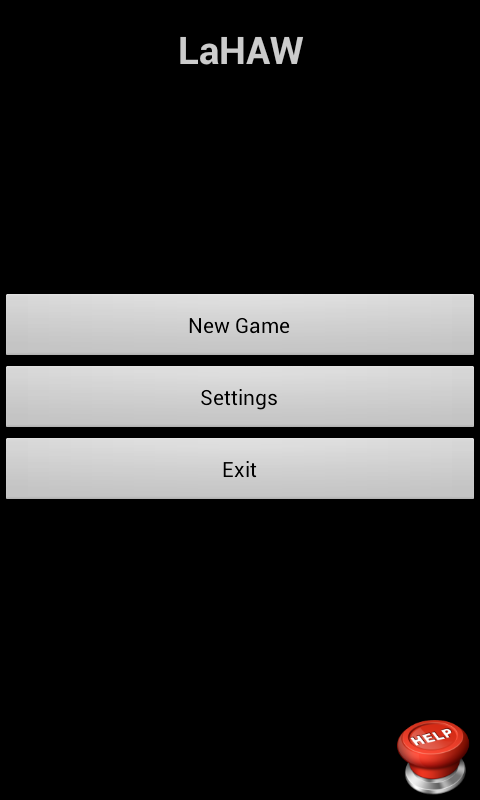
\includegraphics[width=\textwidth]{img/Screenshot_MainMenu.png}
    \caption{The game's main menu}
    \label{fig:Screenshot_MainMenu}
\end{figure}


From the main menu, the player can exectute three actions: \emph{start a new game}; \emph{edit game settings}, including player name and boat colour; and ask the system for \emph{help}\footnote{Note: the hint system is as of this prototype version implemented, but does not contain any actual hints at this time.}.

At the settings screen (see figure \ref{fig:settings}), players of the game can register their name, and preferred boat colour\footnote{Note: the boat colour is not used for anything in this prototype, but is stored on the device for future development of the application.}. 

When a player starts a game, he can select a difficulty. In this version of the game, the difficulty dictates the size of the opponent's game board, with the easiest game mode having the least amount of bombable tiles than the harder modes. This setting is asymmetrical between the players.

The warships are placed on preliminary positions at the start of the game. The players then change the placement by dragging the ships to their new location. Rotation of the warships is done by holding a ship, and then touching the screen with another finger\footnote{We realise that this is a horrendous way to accomplish the action, but it has been left in due to time constraints.}. After the player is happy with the placements, the game is started by pressing the "Start game" button in the upper left corner of the screen.

The game itself is done in turns. Each of the players gets their turn to guess the loacation of their opponent's warships. By tapping the screen on the desired location, a guess is made. If the opponent has a warship that occupies this location, a hit is registered and displayed on the screen (see figure \ref{fig:warship_bombed}). When the whole warship is completely bombed, the entire warship is revealed (see figure \ref{fig:warship_sunk}). After a guess has been made, the table switches, and the opponent gets to guess a position. After an entire fleet has been demolished, the player with remaining warships is declared the winner (see figure \ref{fig:winner}. The user then accepts this outcome, and the game goes back to the main menu.

If the player wants to prematurely end a game, the game can be paused by pressing the "Pause game" button at the upper left corner of the screen. This will pause the game, and present the player with two choices: resume the current game; and exit the current game. Exiting the game will bring the player to the game's main menu screen.